\documentclass[11pt]{article}
\usepackage{fullpage,amsmath}
\usepackage{amssymb,verbatim}
\thispagestyle{empty}

\usepackage{graphicx,amsmath,color,amssymb}
\usepackage{psfrag,picture}

\newcommand{\ba}{\begin{array}}
\newcommand{\ea}{\end{array}}
\newcommand{\be}{\begin{equation}}
\newcommand{\ee}{\end{equation}}
\newcommand{\bd}{\begin{displaymath}}
\newcommand{\ed}{\end{displaymath}}
\newcommand{\bi}{\begin{itemize}}
\newcommand{\ei}{\end{itemize}}
\newcommand{\bn}{\begin{enumerate}}
\newcommand{\en}{\end{enumerate}}
\newcommand{\pa}{\partial}
\newcommand{\f}{\frac}
\newcommand{\ci}{\cite}
\newcommand{\eps}{\epsilon}
\newcommand{\del}{\delta}
%\newcommand{\cal}{\mathcal}
\newtheorem{lem}{Lemma}
\newtheorem{truth}{Theorem}
\newtheorem{prob}{Problem}
\newtheorem{corl}{Corollary}
\newtheorem{rem}{Remark}
\newcommand{\dbl}{[[}
\newcommand{\dbr}{]]}
\newcommand{\dsl}{\{\{}
\newcommand{\dsr}{\}\}} 

\begin{document}
\begin{center}
\textbf{APPM 4720 / 5720 --- HOMEWORK  \# 5\hfill Due: March 1, 2018.}
\end{center}

\subsubsection*{Instructions}
Put away your cell-phone and read this document from start to finish. Discuss in the group what the different instructions and tasks mean. Make sure you have a plan how to achieve the main task (and write up the results!) within the allotted time (team-work is probably needed). How will you check that the subtasks are correct?      

\subsubsection*{Main task}
In this homework we will study how to perform surface and line integrals on a general geometry.  

\begin{enumerate}
\item Find the mapping $(x(r,s),y(r,s))$ that, given the coordinates \mbox{$p_l, \, l = 1,2,3,4$}, maps the reference square $(r,s) \in [-1,1]^2$ into a straight-sided quad (see Figure \ref{fig:map}) in the $x-y$ plane. Hint: for each corner, find a bi-linear function that is one in one corner and zero in all other corners in the $r-s$ plane, and add them up. Check that the mapping is correct by discretizing the reference element by a uniform Cartesian grid and plot the mapped quadrilateral in Matlab by: \verb+plot(x,y,'k',x',y','k'), axis equal+.  

\begin{figure}[ht]
\begin{center}
\setlength{\unitlength}{1.0cm} 
\begin{picture}(8,5) 

\put(0,1.5){\vector(0,1){2}}
\put(0,1.5){\vector(1,0){2}}

\put(5.5,1.5){\vector(0,1){2}}
\put(5.5,1.5){\vector(1,0){2}}

\put(4.5,0.5){\color{blue}{\line(0,1){2}}}
\put(6.5,0.5){\color{blue}{\line(0,1){2}}}
\put(4.5,2.5){\color{blue}{\line(1,0){2}}}
\put(4.5,0.5){\color{blue}{\line(1,0){2}}}

\put(7.5,1.6){$r$}
\put(5.6,3.4){$s$}

\put(2.0,1.6){$x$}
\put(0.1,3.4){$y$}

\put(0.25,2.0){\color{blue}{\line(1,2){1}}}
\put(1.25,4){\color{blue}{\line(2,1){1}}}
\put(2.25,4.5){\color{blue}{\line(1,-3){0.615}}}
\put(0.25,2.0){\color{blue}{\line(4,1){2.61}}}


\put(0.1,1.7){$p_1$}
\put(2.9,2.5){$p_2$}
\put(2.1,4.7){$p_3$}
\put(0.8,4.0){$p_4$}

\put(4.1,0.4){$p'_1$}
\put(6.6,0.4){$p'_2$}
\put(4.1,2.4){$p'_4$}
\put(6.6,2.4){$p'_3$}


\end{picture}
\caption{\label{fig:map}}
\end{center}
\end{figure}

\item To compute integrals of the type $\iint f(x,y) dx dy $ we use the change of variables 
\[
x = x(r,s),\ \ y = x(r,s),
\]
and find that 
 \[
 \iint f(x,y) dx dy = \iint f(x(r,s),x(r,s)) | J | dr ds. 
 \]
 Here 
 \[
  | J | = \left| \left[  \begin{array}{cc}
  \frac{\partial x}{\partial r} & \frac{\partial x}{\partial s} \\
  \frac{\partial y}{\partial r} & \frac{\partial y}{\partial s}
   \end{array} \right] \right|.
  \]
Convince yourself that the formulas are correct by integrating (by iterated 1D Gauss quadrature) the area of a grid like the one displayed in Figure \ref{Fig:Grid}.
\begin{figure}[h]
  \begin{center}
  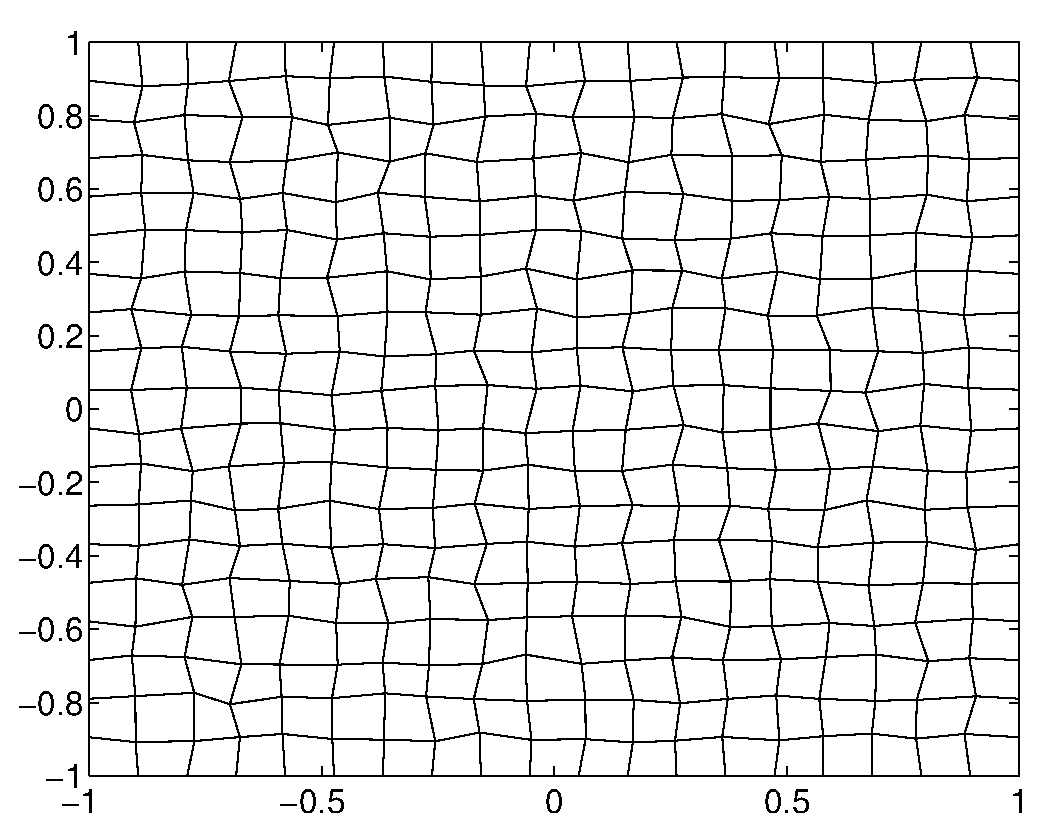
\includegraphics[width=0.5\textwidth]{grid} 
  \caption{Grid made up of uniform Cartesian grid with the interior grid points randomly perturbed. \label{Fig:Grid}}
  \end{center}
\end{figure}
Report how the convergence depends on the quadrature for the 1D integrals, as well as on the total number of cells in the grid.


\item Also compute the area of the half annulus defined by the grid:
\begin{verbatim}
nr = 10; nt = 30; 
[r,theta] = meshgrid(linspace(0.5,1,nr),linspace(0,pi,nt));
x = r.*cos(theta); y = r.*sin(theta); 
plot(x,y,'k',x',y','k'), axis equal
\end{verbatim}

Why is it that the error converges as $\sim (\min (n_r,n_t))^{-2} $ independent of your choice of quadrature? 

\item The mapping you used above does not respect the fact that two of the boundaries of the half annulus are curved. To compute integrals on domains with curved boundaries you will need to use a curvilinear mapping. 

Consider a general quadrilateral with curved boundaries parametrized so that you can use the Gordon-Hall mapping (see equation (8.8.23) in {\it Spectral Methods: Evolution to Complex Geometries and Applications to Fluid Dynamics}, Claudio Canuto, Alfio Quarteroni, M. Yousuff Hussaini, Thomas A. Zang Jr. This book is available electronically from the library).

It will be convenient to have a subroutine (for example called \verb+pis+) that takes as inputs the start and endpoints of a given curve,  \verb+xy_start(1:2)+, \verb+xy_end(1:2)+, and a scalar, \verb+m+ between -1 and 1 that corresponds to the position on an edge of the unit square. The subroutine should also take an integer input, \verb+curve_type+, that can be used to select different type of mappings. The subroutine then computes the $x-y$ coordinate \verb+xy(1:2)+ corresponding to \verb+m+. For example \verb+curve_type = 0+ could correspond to a straight line and the subroutine would then start with:
\begin{verbatim}
    if (curve_type .eq. 0 ) then 
       ! Straight lines.
       xy = xy_start + 0.5_dp*(1.0_dp + m)*(xy_end - xy_start) 
    elseif (curve_type .eq. 1 ) then 
    ... 
\end{verbatim}

In order to use the mapping to compute integrals (and derivatives) you will need to compute the metric, i.e. $r_x, r_y, s_x, s_y$. Recall that the chain rule for a function of two variables requires that:    
\begin{eqnarray*}
\frac{\partial u(x(r,s),y(r,s))}{\partial x} &=& \frac{\partial r}{\partial x}\frac{\partial u}{\partial r}+\frac{\partial s}{\partial x}\frac{\partial u}{\partial s}, \\
\frac{\partial u(x(r,s),y(r,s))}{\partial y} &=& \frac{\partial r}{\partial y}\frac{\partial u}{\partial r}+\frac{\partial s}{\partial y}\frac{\partial u}{\partial s}. 
\end{eqnarray*}
Find the relation between  $r_x, r_y, s_x, s_y$ and  $x_r, y_r, x_x, y_s$ by substituting $u = x$ and $u=y$ into the above equations. 

To obtain $r_x, r_y, s_x, s_y$ evaluate the map $(x(r,s),y(r,s))$ on the LGL nodes (tensor product) on the reference element and use Bengt's \verb+weights.f+ (in the class repository) to compute $x_r, y_r, x_x, y_s$ at the LGL nodes. Use the relations you just derived to invert the metric.  

Using your curvilinear elements repeat the area computation of the half annulus. Make sure you get spectral convergence for a fixed grid and with increasing number of LGL nodes.

\item Use Green's identity and compute the same area by line integrals around each element. How can you express the unit length normals in terms of the metric? 

\item Next, consider approximation in a tensor product polynomial basis expressed in Legendre polynomials. That is, find the the coefficients of an element wise approximation  
\begin{eqnarray}
u^h(x(r,s),y(r,s)) &=& \sum_{k = 0}^{q} \sum_{k = 0}^{q} \hat{u}^h_{k,l} P_k(r) P_l(s), \label{eq:exp} 
\end{eqnarray} 
by $L_2$ projection of some initial data. 

\item Finally, compute $u^h_x = r_x u^h_r + s_x u_s^h$ and  $u^h_y = r_y u^h_r + s_y u_s^h$ on a single element by differentiating the expansion (\ref{eq:exp}). 
\end{enumerate}

For the report make sure you present evidence (convergence plots) that your implementation is correct. 

\end{document}
